% ==============================================================================
% RoadFury — SDC Test Prioritizer | ICST/SBFT 2026 Competition
% LaTeX Beamer Presentation
% Author: Chi-Nguyen Tran
% ==============================================================================
\documentclass[aspectratio=169, 11pt]{beamer}

% ---- Theme & Colors ----
\usetheme{Madrid}
\usecolortheme{default}

% Custom color palette
\definecolor{primaryblue}{RGB}{24, 54, 104}
\definecolor{accentblue}{RGB}{51, 102, 187}
\definecolor{lightblue}{RGB}{219, 234, 254}
\definecolor{successgreen}{RGB}{22, 163, 74}
\definecolor{warnorange}{RGB}{234, 138, 0}
\definecolor{dangerred}{RGB}{220, 53, 69}
\definecolor{graytext}{RGB}{107, 114, 128}
\definecolor{darkbg}{RGB}{30, 41, 59}

\setbeamercolor{palette primary}{bg=primaryblue, fg=white}
\setbeamercolor{palette secondary}{bg=accentblue, fg=white}
\setbeamercolor{palette tertiary}{bg=primaryblue, fg=white}
\setbeamercolor{structure}{fg=primaryblue}
\setbeamercolor{title}{fg=white, bg=primaryblue}
\setbeamercolor{frametitle}{fg=white, bg=primaryblue}
\setbeamercolor{block title}{bg=accentblue, fg=white}
\setbeamercolor{block body}{bg=lightblue, fg=black}
\setbeamercolor{block title alerted}{bg=dangerred, fg=white}
\setbeamercolor{block body alerted}{bg=dangerred!10, fg=black}
\setbeamercolor{block title example}{bg=successgreen, fg=white}
\setbeamercolor{block body example}{bg=successgreen!10, fg=black}
\setbeamercolor{item}{fg=accentblue}

% Remove navigation symbols
\setbeamertemplate{navigation symbols}{}
\setbeamertemplate{footline}{
  \leavevmode%
  \hbox{%
    \begin{beamercolorbox}[wd=.333333\paperwidth,ht=2.25ex,dp=1ex,center]{author in head/foot}%
      \usebeamerfont{author in head/foot}\insertshortauthor
    \end{beamercolorbox}%
    \begin{beamercolorbox}[wd=.333333\paperwidth,ht=2.25ex,dp=1ex,center]{title in head/foot}%
      \usebeamerfont{title in head/foot}\insertshorttitle
    \end{beamercolorbox}%
    \begin{beamercolorbox}[wd=.333333\paperwidth,ht=2.25ex,dp=1ex,right]{date in head/foot}%
      \usebeamerfont{date in head/foot}\insertshortdate{}\hspace*{2em}
      \insertframenumber{} / \inserttotalframenumber\hspace*{2ex}
    \end{beamercolorbox}}%
  \vskip0pt%
}

% ---- Packages ----
\usepackage{fontspec}
\setmainfont{Latin Modern Roman}
\setsansfont{Latin Modern Sans}
\setmonofont{Latin Modern Mono}
\usepackage{amsmath, amssymb}
\usepackage{booktabs}
\usepackage{multirow}
\usepackage{graphicx}
\graphicspath{{figures/}}
\usepackage{tikz}
\usetikzlibrary{arrows.meta, positioning, shapes.geometric, calc, fit, backgrounds}
\usepackage{pgfplots}
\pgfplotsset{compat=1.18}
\usepackage{listings}
\usepackage{xcolor}
\usepackage{fontawesome5}
\usepackage{hyperref}
\usepackage{array}
\usepackage{colortbl}

% Listings style
\lstset{
  basicstyle=\ttfamily\scriptsize,
  keywordstyle=\color{accentblue}\bfseries,
  commentstyle=\color{graytext}\itshape,
  stringstyle=\color{successgreen},
  frame=none,
  backgroundcolor=\color{lightblue!30},
  breaklines=true,
  showstringspaces=false
}

% ---- Metadata ----
\title[RoadFury]{RoadFury: Transformer-Based Test Prioritization\\for Self-Driving Cars in Simulation}
\subtitle{SDC Testing Competition --- ICST/SBFT 2026}
\author[Chi-Nguyen Tran]{Chi-Nguyen Tran}
\institute{
  \href{mailto:tcnguyen2365@gmail.com}{\faEnvelope\ tcnguyen2365@gmail.com}
  \quad
  \href{https://github.com/chisngyen}{\faGithub\ chisngyen}
}
\date{2025}

% ==============================================================================
\begin{document}

% ---- Title Slide ----
{
\setbeamertemplate{footline}{}
\begin{frame}[plain]
\begin{tikzpicture}[remember picture, overlay]
  % Background gradient
  \fill[primaryblue] (current page.south west) rectangle (current page.north east);
  \fill[accentblue, opacity=0.3] (current page.south west) -- ++(0,4) -- ++(16,2) -- ++(0,-6) -- cycle;
  \fill[white, opacity=0.05] (current page.north west) -- ++(8,-3) -- ++(8,1) -- ++(0,2) -- cycle;
  
  % Title content
  \node[white, anchor=west, font=\Huge\bfseries, text width=13cm] at ([xshift=1.2cm, yshift=1.5cm]current page.west) {RoadFury};
  \node[white, anchor=west, font=\large, text width=13cm] at ([xshift=1.2cm, yshift=0.5cm]current page.west) {Transformer-Based Test Prioritization for Self-Driving Cars};
  
  % Separator line
  \draw[warnorange, line width=2pt] ([xshift=1.2cm, yshift=-0.2cm]current page.west) -- ++(5,0);
  
  % Subtitle
  \node[lightblue, anchor=west, font=\normalsize] at ([xshift=1.2cm, yshift=-0.9cm]current page.west) {SDC Testing Competition --- ICST/SBFT 2026};
  \node[lightblue, anchor=west, font=\normalsize] at ([xshift=1.2cm, yshift=-1.5cm]current page.west) {Daejeon, Republic of Korea};
  
  % Author info
  \node[white, anchor=west, font=\small] at ([xshift=1.2cm, yshift=-2.3cm]current page.west) 
    {Trần Chí Nguyên* \quad Đào Sỹ Duy Minh* \quad Huỳnh Trung Kiệt*};
  \node[white, anchor=west, font=\small] at ([xshift=1.2cm, yshift=-2.9cm]current page.west) 
    {Phạm Phú Hòa \quad Nguyễn Lâm Phú Quý};
\end{tikzpicture}
\end{frame}
}

% ---- Outline ----
\begin{frame}{Outline}
\tableofcontents
\end{frame}

% ==============================================================================
\section{Introduction}
% ==============================================================================

\begin{frame}{Motivation: Testing Self-Driving Cars}
% --- Top: bullet points + diagram side by side ---
\begin{columns}[T]
\begin{column}{0.52\textwidth}
  \begin{itemize}
    \item Self-driving cars (SDCs) require \textbf{extensive simulation testing}
    \item Each simulation test is \textbf{computationally expensive}
    \item Real-world safety depends on thorough testing coverage
    \item \textbf{Key challenge:} Run the most failure-revealing tests \emph{first}
  \end{itemize}
\end{column}
\begin{column}{0.45\textwidth}
  \centering
  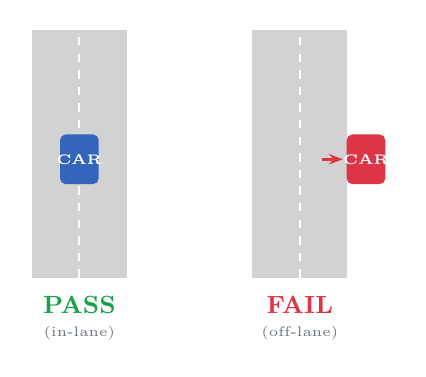
\begin{tikzpicture}[scale=0.7]
    % === PASS road (left) ===
    % Road edges
    \fill[gray!35] (-0.9,0) rectangle (0.9,4.5);
    \draw[white, line width=1.5pt] (-0.9,0) -- (-0.9,4.5);
    \draw[white, line width=1.5pt] (0.9,0) -- (0.9,4.5);
    % Center dashed line
    \draw[white, dashed, line width=0.8pt] (0,0) -- (0,4.5);
    % Car (centered on road)
    \fill[accentblue, rounded corners=2pt] (-0.35,1.7) rectangle (0.35,2.6);
    \node[font=\tiny\bfseries, white] at (0,2.15) {CAR};
    % Label
    \node[font=\small\bfseries, successgreen] at (0, -0.5) {PASS};
    \node[font=\tiny, graytext] at (0, -1.0) {(in-lane)};
    
    % === FAIL road (right) ===
    \fill[gray!35] (3.1,0) rectangle (4.9,4.5);
    \draw[white, line width=1.5pt] (3.1,0) -- (3.1,4.5);
    \draw[white, line width=1.5pt] (4.9,0) -- (4.9,4.5);
    \draw[white, dashed, line width=0.8pt] (4,0) -- (4,4.5);
    % Car (off-road to the right)
    \fill[dangerred, rounded corners=2pt] (4.85,1.7) rectangle (5.55,2.6);
    \node[font=\tiny\bfseries, white] at (5.2,2.15) {CAR};
    % Arrow showing drift
    \draw[dangerred, -{Stealth[length=5pt]}, very thick] (4.4,2.15) -- (4.78,2.15);
    % Label
    \node[font=\small\bfseries, dangerred] at (4, -0.5) {FAIL};
    \node[font=\tiny, graytext] at (4, -1.0) {(off-lane)};
  \end{tikzpicture}
\end{column}
\end{columns}

\vspace{0.4em}
% --- Bottom: full-width block ---
\begin{block}{Test Outcome Definition}
  \begin{description}
    \item[\textcolor{successgreen}{PASS}] Car stays \textbf{within the lane} throughout the simulation scenario
    \item[\textcolor{dangerred}{FAIL}] Car drives \textbf{off the lane} during simulation $\rightarrow$ test execution stops immediately
  \end{description}
\end{block}
\end{frame}

% ---- Competition Overview ----
\begin{frame}{SDC Testing Competition 2026}
\begin{columns}[T]
\begin{column}{0.54\textwidth}
  \begin{block}{Competition Details}
    \begin{itemize}
      \item \textbf{Focus:} Test Prioritization for SDCs
      \item \textbf{Simulator:} BeamNG.tech
      \item \textbf{Interface:} gRPC (language-agnostic)
      \item \textbf{Deployment:} Docker container
      \item \textbf{Metric:} Average Percentage of Faults Detected (APFD)
    \end{itemize}
  \end{block}
\end{column}
\begin{column}{0.44\textwidth}
  \begin{block}{gRPC Interface}
    \centering
    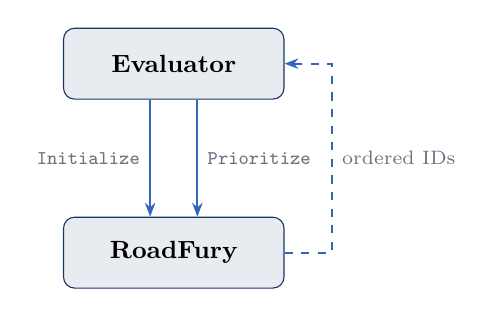
\begin{tikzpicture}[
      box/.style={draw=primaryblue, fill=primaryblue!10, rounded corners=4pt, 
                  minimum width=2.8cm, minimum height=0.9cm, font=\small\bfseries,
                  align=center},
      arr/.style={-{Stealth[length=5pt]}, accentblue, thick}
    ]
      \node[box] (eval) at (0,0) {Evaluator};
      \node[box] (tool) at (0,-2.4) {RoadFury};
      
      \draw[arr] ([xshift=-3mm]eval.south) -- node[left, font=\scriptsize, text=graytext] {\texttt{Initialize}} ([xshift=-3mm]tool.north);
      \draw[arr] ([xshift=3mm]eval.south) -- node[right, font=\scriptsize, text=graytext] {\texttt{Prioritize}} ([xshift=3mm]tool.north);
      \draw[arr, dashed] (tool.east) -- ++(0.6,0) |- node[right, font=\scriptsize, pos=0.25, text=graytext] {ordered IDs} (eval.east);
    \end{tikzpicture}
  \end{block}
\end{column}
\end{columns}

\vspace{0.3em}
\begin{block}{Venues}
  \begin{itemize}
    \item \textbf{ICST 2026} --- Daejeon, South Korea
    \item \textbf{SBFT 2026} --- Rio de Janeiro, Brazil
  \end{itemize}
\end{block}
\end{frame}

% ---- APFD Metric ----
\begin{frame}{Evaluation Metric: APFD}
\begin{columns}[T]
\begin{column}{0.50\textwidth}
  \begin{block}{Average Percentage of Faults Detected}
    \vspace{0.3em}
    $$\text{APFD} = 1 - \frac{\sum_{i=1}^{m} TF_i}{n \cdot m} + \frac{1}{2n}$$
    \vspace{0.2em}
    \begin{itemize}
      \item $n$ = total number of test cases
      \item $m$ = number of faulty test cases
      \item $TF_i$ = position of the $i$-th fault in the order
    \end{itemize}
  \end{block}
\end{column}
\begin{column}{0.47\textwidth}
  \centering
  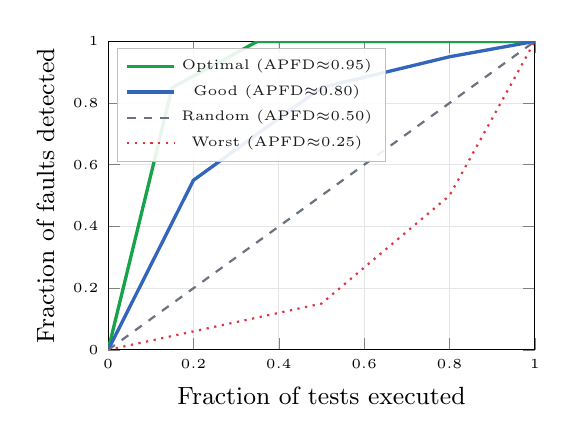
\begin{tikzpicture}
    \begin{axis}[
      width=7cm, height=5.5cm,
      xlabel={Fraction of tests executed},
      ylabel={Fraction of faults detected},
      xmin=0, xmax=1, ymin=0, ymax=1,
      grid=major, grid style={gray!20},
      legend style={at={(0.02,0.98)}, anchor=north west, font=\tiny,
                    fill=white, fill opacity=0.9, draw=gray!50},
      xlabel style={font=\small},
      ylabel style={font=\small},
      tick label style={font=\tiny}
    ]
      % Optimal
      \addplot[successgreen, very thick] coordinates {(0,0) (0.15,0.85) (0.35,1.0) (1,1)};
      \addlegendentry{Optimal (APFD$\approx$0.95)}
      % Good prioritizer
      \addplot[accentblue, very thick] coordinates {(0,0) (0.2,0.55) (0.5,0.85) (0.8,0.95) (1,1)};
      \addlegendentry{Good (APFD$\approx$0.80)}
      % Random
      \addplot[graytext, thick, dashed] coordinates {(0,0) (1,1)};
      \addlegendentry{Random (APFD$\approx$0.50)}
      % Bad
      \addplot[dangerred, thick, dotted] coordinates {(0,0) (0.5,0.15) (0.8,0.5) (1,1)};
      \addlegendentry{Worst (APFD$\approx$0.25)}
    \end{axis}
  \end{tikzpicture}
\end{column}
\end{columns}
\end{frame}

% ==============================================================================
\section{Dataset}
% ==============================================================================

\begin{frame}{Training Data: SensoDat}
\begin{columns}[T]
\begin{column}{0.50\textwidth}
  \textbf{\large SensoDat Dataset}
  \vspace{0.3em}
  \begin{itemize}
    \item \textbf{36,006} labeled simulation tests
    \item Extracted from \textbf{.xodr} road files
    \item Each test: sequence of 2D road points
    \item Labels: \texttt{PASS} or \texttt{FAIL}
  \end{itemize}
  
  \vspace{0.3em}
  \begin{block}{Data Split}
    \centering
    \begin{tabular}{lrrr}
      \toprule
      \textbf{Split} & \textbf{Total} & \textbf{FAIL} & \textbf{FAIL \%} \\
      \midrule
      Train & 28,804 & 11,059 & 38.4\% \\
      Test  & 7,202  & 2,765  & 38.4\% \\
      \midrule
      \textbf{Total} & \textbf{36,006} & \textbf{13,824} & \textbf{38.4\%} \\
      \bottomrule
    \end{tabular}
  \end{block}
\end{column}
\begin{column}{0.47\textwidth}
  \begin{block}{Test Case = Road Geometry}
    \centering
    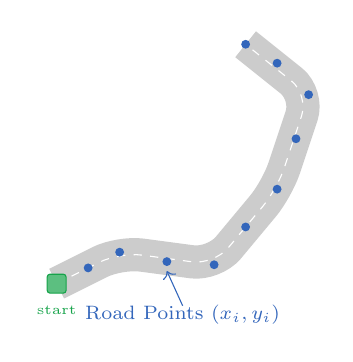
\begin{tikzpicture}[scale=0.8]
      % Draw a curved road
      \draw[gray!40, line width=12pt, rounded corners=8pt] 
        (0,0) -- (1,0.5) -- (2.5,0.3) -- (3.5,1.5) -- (4,3) -- (3,3.8);
      % Road center line
      \draw[white, dashed, line width=0.4pt, rounded corners=8pt] 
        (0,0) -- (1,0.5) -- (2.5,0.3) -- (3.5,1.5) -- (4,3) -- (3,3.8);
      % Road points
      \foreach \x/\y in {0/0, 0.5/0.25, 1/0.5, 1.75/0.35, 2.5/0.3, 3/0.9, 3.5/1.5, 3.8/2.3, 4/3, 3.5/3.5, 3/3.8} {
        \fill[accentblue] (\x,\y) circle (2pt);
      }
      % Car start
      \draw[successgreen, fill=successgreen!70, rounded corners=1pt] (-0.15,-0.15) rectangle (0.15,0.15);
      \node[font=\tiny, successgreen, below] at (0,-0.2) {start};
      
      % Labels
      \node[font=\scriptsize, accentblue] at (2, -0.5) {Road Points $(x_i, y_i)$};
      \draw[->, accentblue, thin] (2,-0.35) -- (1.75,0.2);
    \end{tikzpicture}
  \end{block}
  
  \vspace{0.3em}
  {\small\textbf{Competition Evaluation:} Evaluated on \textbf{956 competition tests} (353 FAIL)
  with \textbf{30-trial random subsampling} (287 tests each)}
\end{column}
\end{columns}
\end{frame}

% ==============================================================================
\section{Approach}
% ==============================================================================

\begin{frame}{RoadFury: Approach Overview}
\centering
\begin{tikzpicture}[
  block/.style={draw=primaryblue, fill=primaryblue!8, rounded corners=5pt,
                minimum height=1.2cm, text width=2.8cm, align=center,
                font=\small\bfseries},
  arrow/.style={-{Stealth[length=6pt]}, primaryblue, thick},
  label/.style={font=\tiny, text=graytext, align=center}
]
  % Input
  \node[block, fill=lightblue] (input) at (0,0) {Road Points\\$(x_i, y_i)$};
  
  % Feature extraction
  \node[block, fill=warnorange!15, draw=warnorange] (feat) at (3.5,0) {10-Channel\\Features};
  
  % Transformer
  \node[block, fill=accentblue!15, draw=accentblue, text width=3.2cm] (trans) at (7.5,0) {Transformer\\Encoder\\{\scriptsize (4L, 8H, d=128)}};
  
  % Output
  \node[block, fill=successgreen!15, draw=successgreen] (out) at (11.5,0) {P(FAIL)\\Score};
  
  % Arrows
  \draw[arrow] (input) -- node[above, label] {extract} (feat);
  \draw[arrow] (feat) -- node[above, label] {normalize} (trans);
  \draw[arrow] (trans) -- node[above, label] {sigmoid} (out);
  
  % Training techniques below
  \node[draw=warnorange, fill=warnorange!10, rounded corners=3pt, 
        font=\scriptsize\bfseries, inner sep=4pt] (swa) at (5.5,-2) 
    {\faSync\ SWA (epoch 50--75)};
  \node[draw=dangerred, fill=dangerred!10, rounded corners=3pt,
        font=\scriptsize\bfseries, inner sep=4pt] (focal) at (9.5,-2) 
    {\faBullseye\ Focal Loss ($\gamma$=2.5)};
  
  \draw[warnorange, dashed, thick, ->] (swa) -- (trans);
  \draw[dangerred, dashed, thick, ->] (focal) -- (out);
\end{tikzpicture}
\end{frame}

% ---- 10-Channel Features ----
\begin{frame}{Feature Engineering: 10-Channel Road Geometry}
\begin{columns}[T]
\begin{column}{0.48\textwidth}
  \begin{block}{Feature Channels}
    \centering
    \small
    \renewcommand{\arraystretch}{1.15}
    \begin{tabular}{cl}
      \toprule
      \textbf{Ch} & \textbf{Feature} \\
      \midrule
      0 & Segment length \\
      1 & Absolute angle change \\
      2 & Menger curvature \\
      3 & Curvature jerk (1st deriv.) \\
      4 & Cumulative dist. (norm.) \\
      5 & Heading $\sin(\theta)$ \\
      6 & Heading $\cos(\theta)$ \\
      7 & Relative position \\
      8 & Local curvature std ($w$=11) \\
      9 & Curvature accel. (2nd deriv.) \\
      \bottomrule
    \end{tabular}
  \end{block}
\end{column}
\begin{column}{0.49\textwidth}
    \begin{itemize}
      \item \textbf{Geometry}: Curvature, jerk, acceleration capture road \emph{difficulty}
      \item \textbf{Direction}: $(sin, cos)$ heading avoids angle discontinuities
      \item \textbf{Context}: Local std captures \emph{variability} of curvature
      \item \textbf{Position}: Relative position and cumulative distance add \emph{spatial context}
    \end{itemize}
  
  \vspace{0.3em}
  \textbf{Preprocessing}
  \begin{itemize}
    \item Interpolate to \textbf{197 points} (standard length)
    \item Per-channel z-score normalization
    \item Input shape: $[B, 10, 197]$
  \end{itemize}
\end{column}
\end{columns}
\end{frame}

% ---- Model Architecture (image) ----
\begin{frame}{Model Architecture: Road Transformer}
\centering
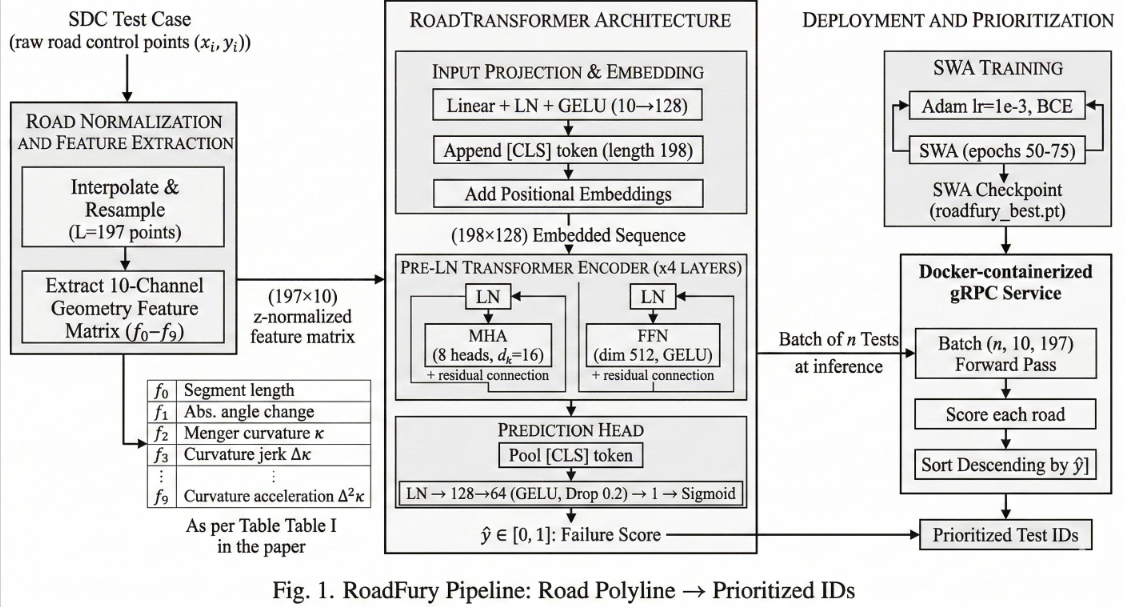
\includegraphics[width=0.85\textwidth, height=0.82\textheight, keepaspectratio]{pipeline.png}
\end{frame}

% ---- SWA ----
\begin{frame}{Stochastic Weight Averaging (SWA)}
\begin{columns}[T]
\begin{column}{0.52\textwidth}
  \begin{block}{Key Idea [Izmailov et al., 2018]}
    \begin{itemize}
      \item Average model weights over final training epochs
      \item Converges to \textbf{flatter minima} in loss landscape
      \item Flatter minima $\rightarrow$ \textbf{better generalization}
      \item Simple yet effective regularization technique
    \end{itemize}
  \end{block}
  
  \vspace{0.3em}
  \textbf{Our Configuration}
  \begin{itemize}
    \item Total training: \textbf{75 epochs}
    \item SWA collection: \textbf{epoch 50--75}
    \item 24 weight snapshots averaged
  \end{itemize}

\end{column}
\begin{column}{0.45\textwidth}
  \centering
  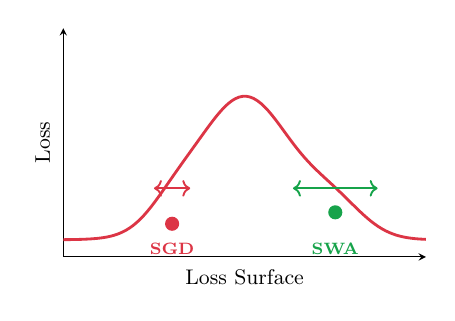
\begin{tikzpicture}[scale=0.85]
    \begin{axis}[
      width=7cm, height=5cm,
      xlabel={Loss Surface},
      ylabel={Loss},
      xmin=-3, xmax=3, ymin=0, ymax=4,
      xtick=\empty, ytick=\empty,
      axis lines=left,
      xlabel style={font=\small},
      ylabel style={font=\small}
    ]
      % Sharp minimum (SGD)
      \addplot[dangerred, very thick, domain=-3:3, samples=100] 
        {0.3*exp(-3*(x+1.2)^2) + 2.5*exp(-0.8*(x)^2) + 0.5*exp(-2*(x-1.5)^2) + 0.3};
      
      % Mark sharp vs flat
      \node[dangerred, font=\scriptsize\bfseries] at (axis cs:-1.2,0.15) {SGD};
      \node[font=\tiny, dangerred] at (axis cs:-1.2,-0.3) {sharp};
      \fill[dangerred] (axis cs:-1.2,0.58) circle (3pt);
      
      \node[successgreen, font=\scriptsize\bfseries] at (axis cs:1.5,0.15) {SWA};
      \node[font=\tiny, successgreen] at (axis cs:1.5,-0.3) {flat};
      \fill[successgreen] (axis cs:1.5,0.78) circle (3pt);
      
      % Arrows showing width
      \draw[dangerred, <->, thick] (axis cs:-1.5,1.2) -- (axis cs:-0.9,1.2);
      \draw[successgreen, <->, thick] (axis cs:0.8,1.2) -- (axis cs:2.2,1.2);
    \end{axis}
  \end{tikzpicture}
  
  \vspace{0.3em}
  \begin{exampleblock}{\small Impact}
    SWA alone improved APFD by\\
    \textbf{+0.0143} (0.7899 $\to$ 0.8042)
  \end{exampleblock}
\end{column}
\end{columns}
\end{frame}

% ---- Focal Loss ----
\begin{frame}{Focal Loss for Hard Examples}
\begin{columns}[T]
\begin{column}{0.50\textwidth}
  \begin{block}{Focal Loss [Lin et al., 2017]}
    $$\mathcal{L}_{\text{FL}} = -\alpha (1 - p_t)^\gamma \log(p_t)$$
    \begin{itemize}
      \item Down-weights \textbf{easy} examples ($p_t \approx 1$)
      \item Focuses learning on \textbf{hard, borderline} tests
      \item $\gamma$ controls focusing strength
    \end{itemize}
  \end{block}
\end{column}
\begin{column}{0.47\textwidth}
  \begin{block}{Gamma Sweep Results}
    \centering
    \small
    \begin{tabular}{cc}
      \toprule
      $\gamma$ & \textbf{APFD (SWA)} \\
      \midrule
      0.0 (BCE) & 0.8001 \\
      1.0 & 0.8052 \\
      1.5 & 0.8045 \\
      2.0 & 0.8020 \\
      \rowcolor{successgreen!20} \textbf{2.5} & \textbf{0.8066} \\
      \bottomrule
    \end{tabular}
  \end{block}
\end{column}
\end{columns}
\end{frame}

% ==============================================================================
\section{Experiments}
% ==============================================================================

% ---- Ablation Study ----
\begin{frame}{Ablation Study: Individual Improvements}
\begin{columns}[T]
\begin{column}{0.52\textwidth}
  \begin{exampleblock}{Key Findings}
    \begin{itemize}
      \item SWA is the \textbf{single best} improvement (+1.8\%)
      \item Focal Loss is 2nd best (+0.8\% alone, but \textbf{+2.1\%} with SWA)
      \item Architectural changes (Mixup, DropPath, etc.) \\did \emph{not} help on this task
    \end{itemize}
  \end{exampleblock}
\end{column}
\begin{column}{0.46\textwidth}
  \centering
  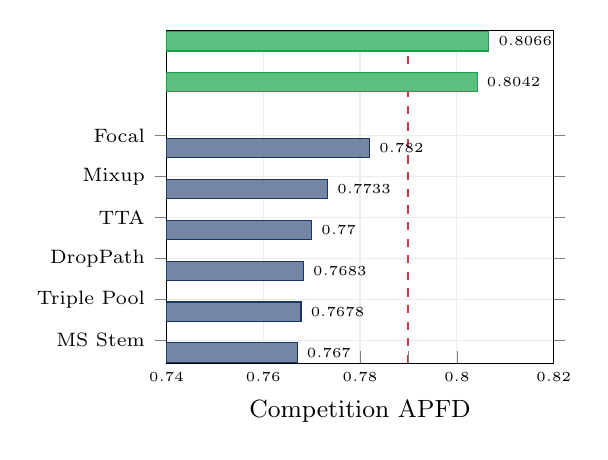
\begin{tikzpicture}
    \begin{axis}[
      xbar, width=6.5cm, height=5.8cm,
      xlabel={Competition APFD},
      xmin=0.74, xmax=0.82,
      symbolic y coords={MS Stem,Triple Pool,DropPath,TTA,Mixup,Focal,SWA,SWA+Focal},
      ytick=data,
      y tick label style={font=\scriptsize},
      x tick label style={font=\tiny},
      xlabel style={font=\small},
      nodes near coords,
      nodes near coords style={font=\tiny, /pgf/number format/fixed, /pgf/number format/precision=4},
      every node near coord/.append style={anchor=west},
      bar width=7pt,
      grid=major, grid style={gray!15},
      xmajorgrids=true,
      extra x ticks={0.7899},
      extra x tick style={grid=major, grid style={dashed, dangerred, thick}},
      extra x tick labels={},
      enlarge y limits=0.08
    ]
      \addplot[fill=primaryblue!60, draw=primaryblue] coordinates {
        (0.7670,MS Stem)
        (0.7678,Triple Pool)
        (0.7683,DropPath)
        (0.7700,TTA)
        (0.7733,Mixup)
        (0.7820,Focal)
      };
      \addplot[fill=successgreen!70, draw=successgreen] coordinates {
        (0.8042,SWA)
        (0.8066,SWA+Focal)
      };
    \end{axis}
  \end{tikzpicture}
\end{column}
\end{columns}
\end{frame}

% ==============================================================================
\section{Results}
% ==============================================================================

% ---- Multi-Paradigm Comparison ----
\begin{frame}{Why Transformers? Multi-Paradigm Exploration}
\begin{columns}[T]
\begin{column}{0.52\textwidth}
  \centering
  \renewcommand{\arraystretch}{1.2}
  \small
  \begin{tabular}{l c c}
    \toprule
    \textbf{Method} & \textbf{Paradigm} & \textbf{APFD} \\
    \midrule
    Random & --- & 0.493 \\
    LLM zero-shot & Qwen2.5-7B, 4-bit & 0.487{\tiny$\pm$.019} \\
    GNN & 3-layer GCN+KNN & 0.533{\tiny$\pm$.025} \\
    ResNet50+XGB & Road image CNN & 0.572{\tiny$\pm$.013} \\
    CNN+Handcraft & ResNet50+44 feat. & 0.673{\tiny$\pm$.017} \\
    ExtCNN-10ch & 10-ch CNN, 28K & 0.768{\tiny$\pm$.014} \\
    \midrule
    ITEP4SDC & ONNX MLP, 3 feat. & 0.781 \\
    \rowcolor{successgreen!20}
    \textbf{RoadFury} & \textbf{Transformer+SWA} & \textbf{0.804{\tiny$\pm$.012}} \\
    \bottomrule
  \end{tabular}
\end{column}
\begin{column}{0.45\textwidth}
  \begin{alertblock}{\small LLMs fail at geometry}
    \small Language models can discuss curves but cannot judge whether a specific curvature value is dangerous.
  \end{alertblock}
  
  \vspace{0.2em}
  \begin{block}{\small Graphs lose the sequence}
    \small GCN captures local neighborhoods but discards \emph{ordering}---a sharp turn after a straight is more dangerous than after a gradual curve.
  \end{block}
  
  \vspace{0.2em}
  \begin{exampleblock}{\small Insight}
    \small \textbf{What you measure} matters more than \textbf{how you model it}: 10-ch features in a simple CNN already reach 0.768.
  \end{exampleblock}
\end{column}
\end{columns}
\end{frame}

% ---- Main Results ----
\begin{frame}{Results: RoadFury vs.\ Existing Tools}
\vspace{-0.5em}
\begin{center}
  \renewcommand{\arraystretch}{1.3}
  \small
  \begin{tabular}{l c c c}
    \toprule
    \textbf{Tool} & \textbf{Method} & \textbf{APFD} & \textbf{vs.\ Random} \\
    \midrule
    \rowcolor{successgreen!20}
    \textbf{RoadFury (Ours)} & \textbf{Transformer + SWA + Focal} & \textbf{0.8066 $\pm$ 0.0124} & \textbf{+62.6\%} \\
    \rowcolor{successgreen!8}
    \quad \emph{Ensemble 5$\times$SWA} & \emph{Multi-gamma average} & \emph{0.8077 $\pm$ 0.0115} & \emph{+63.8\%} \\
    \midrule
    ITEP4SDC & ONNX classifier & 0.7812 & +58.5\% \\
    RoadFury (old) & 1D-CNN & 0.6487 & +31.6\% \\
    \midrule
    Random baseline & --- & 0.4930 & --- \\
    \bottomrule
  \end{tabular}
\end{center}

\vspace{0.5em}
\begin{columns}[T]
\begin{column}{0.48\textwidth}
  \begin{exampleblock}{\faCheckCircle\ Key Achievement}
    RoadFury surpasses the previous SOTA (ITEP4SDC)\\
    by \textbf{+0.0254 APFD} (+3.3\% relative)
  \end{exampleblock}
\end{column}
\begin{column}{0.48\textwidth}
  \begin{block}{\faChartBar\ Improvement Breakdown}
    \begin{itemize}
      \item Base Transformer: +0.1412 over old CNN
      \item +SWA: +0.0143 additional
      \item +Focal($\gamma$=2.5): +0.0024 additional
    \end{itemize}
  \end{block}
\end{column}
\end{columns}
\end{frame}

% ==============================================================================
\section{Conclusion}
% ==============================================================================

\begin{frame}{Conclusion \& Contributions}
\begin{columns}[T]
\begin{column}{0.55\textwidth}
  \begin{block}{Summary}
    \begin{enumerate}
      \item \textbf{Novel architecture}: First Transformer-based test prioritizer for SDCs
      \item \textbf{Rich features}: 10-channel road geometry (curvature, jerk, heading, etc.)
      \item \textbf{SWA + Focal Loss}: Simple yet effective training recipe
      \item \textbf{New SOTA}: APFD 0.8066 (+3.3\% over ITEP4SDC)
      \item \textbf{Practical}: Lightweight (3.2 MB), CPU-only inference
    \end{enumerate}
  \end{block}
\end{column}
\begin{column}{0.42\textwidth}
  \centering
  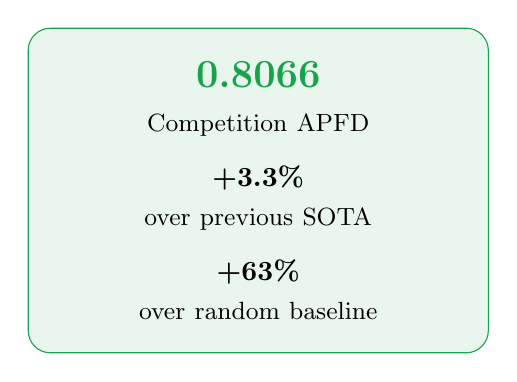
\begin{tikzpicture}
    % Achievement box
    \node[draw=successgreen, fill=successgreen!10, rounded corners=8pt, 
          inner sep=12pt, text width=5cm, align=center] (box) {
      {\Large\bfseries\color{successgreen} 0.8066}\\[4pt]
      {\small Competition APFD}\\[8pt]
      {\normalsize\bfseries +3.3\%}\\[2pt]
      {\small over previous SOTA}\\[8pt]
      {\normalsize\bfseries +63\%}\\[2pt]
      {\small over random baseline}
    };
  \end{tikzpicture}
\end{column}
\end{columns}
\end{frame}

% ---- Thank You ----
{
\setbeamertemplate{footline}{}
\begin{frame}[plain]
\begin{tikzpicture}[remember picture, overlay]
  \fill[primaryblue] (current page.south west) rectangle (current page.north east);
  \fill[accentblue, opacity=0.3] (current page.south east) -- ++(-8,3) -- ++(0,-3) -- cycle;
  
  \node[white, font=\Huge\bfseries] at ([yshift=1.5cm]current page.center) {Thank You!};
  \node[lightblue, font=\large] at ([yshift=0.3cm]current page.center) {Questions?};
  
  \draw[warnorange, line width=2pt] ([yshift=-0.5cm, xshift=-2cm]current page.center) -- ++(4,0);
  
\end{tikzpicture}
\end{frame}
}

\end{document}
